% Created by tikzDevice version 0.12.3 on 2020-09-01 15:22:28
% !TEX encoding = UTF-8 Unicode
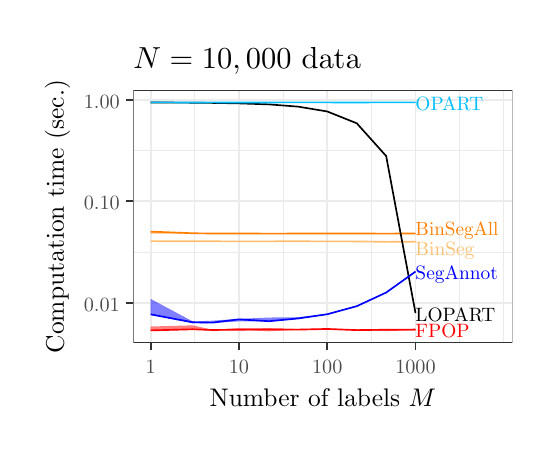
\begin{tikzpicture}[x=1pt,y=1pt]
\definecolor{fillColor}{RGB}{255,255,255}
\path[use as bounding box,fill=fillColor,fill opacity=0.00] (0,0) rectangle (180.67,144.54);
\begin{scope}
\path[clip] (  0.00,  0.00) rectangle (180.67,144.54);
\definecolor{drawColor}{RGB}{255,255,255}
\definecolor{fillColor}{RGB}{255,255,255}

\path[draw=drawColor,line width= 0.6pt,line join=round,line cap=round,fill=fillColor] ( -0.00,  0.00) rectangle (180.67,144.54);
\end{scope}
\begin{scope}
\path[clip] ( 38.23, 30.69) rectangle (175.17,121.88);
\definecolor{fillColor}{RGB}{255,255,255}

\path[fill=fillColor] ( 38.23, 30.69) rectangle (175.17,121.88);
\definecolor{drawColor}{gray}{0.92}

\path[draw=drawColor,line width= 0.3pt,line join=round] ( 38.23, 63.47) --
	(175.17, 63.47);

\path[draw=drawColor,line width= 0.3pt,line join=round] ( 38.23,100.11) --
	(175.17,100.11);

\path[draw=drawColor,line width= 0.3pt,line join=round] ( 60.40, 30.69) --
	( 60.40,121.88);

\path[draw=drawColor,line width= 0.3pt,line join=round] ( 92.30, 30.69) --
	( 92.30,121.88);

\path[draw=drawColor,line width= 0.3pt,line join=round] (124.20, 30.69) --
	(124.20,121.88);

\path[draw=drawColor,line width= 0.3pt,line join=round] (156.09, 30.69) --
	(156.09,121.88);

\path[draw=drawColor,line width= 0.3pt,line join=round] (172.04, 30.69) --
	(172.04,121.88);

\path[draw=drawColor,line width= 0.6pt,line join=round] ( 38.23, 45.15) --
	(175.17, 45.15);

\path[draw=drawColor,line width= 0.6pt,line join=round] ( 38.23, 81.79) --
	(175.17, 81.79);

\path[draw=drawColor,line width= 0.6pt,line join=round] ( 38.23,118.43) --
	(175.17,118.43);

\path[draw=drawColor,line width= 0.6pt,line join=round] ( 44.45, 30.69) --
	( 44.45,121.88);

\path[draw=drawColor,line width= 0.6pt,line join=round] ( 76.35, 30.69) --
	( 76.35,121.88);

\path[draw=drawColor,line width= 0.6pt,line join=round] (108.25, 30.69) --
	(108.25,121.88);

\path[draw=drawColor,line width= 0.6pt,line join=round] (140.14, 30.69) --
	(140.14,121.88);
\definecolor{fillColor}{RGB}{253,191,111}

\path[fill=fillColor,fill opacity=0.50] ( 44.45, 67.45) --
	( 59.67, 67.36) --
	( 66.75, 67.34) --
	( 76.35, 67.34) --
	( 87.27, 67.34) --
	( 97.79, 67.44) --
	(108.25, 67.38) --
	(118.92, 67.33) --
	(129.54, 67.21) --
	(140.14, 67.19) --
	(140.14, 67.11) --
	(129.54, 67.08) --
	(118.92, 67.25) --
	(108.25, 67.24) --
	( 97.79, 67.33) --
	( 87.27, 67.21) --
	( 76.35, 67.23) --
	( 66.75, 67.24) --
	( 59.67, 67.31) --
	( 44.45, 67.40) --
	cycle;

\path[] ( 44.45, 67.45) --
	( 59.67, 67.36) --
	( 66.75, 67.34) --
	( 76.35, 67.34) --
	( 87.27, 67.34) --
	( 97.79, 67.44) --
	(108.25, 67.38) --
	(118.92, 67.33) --
	(129.54, 67.21) --
	(140.14, 67.19);

\path[] (140.14, 67.11) --
	(129.54, 67.08) --
	(118.92, 67.25) --
	(108.25, 67.24) --
	( 97.79, 67.33) --
	( 87.27, 67.21) --
	( 76.35, 67.23) --
	( 66.75, 67.24) --
	( 59.67, 67.31) --
	( 44.45, 67.40);
\definecolor{fillColor}{RGB}{255,127,0}

\path[fill=fillColor,fill opacity=0.50] ( 44.45, 70.87) --
	( 59.67, 70.34) --
	( 66.75, 70.19) --
	( 76.35, 70.21) --
	( 87.27, 70.22) --
	( 97.79, 70.15) --
	(108.25, 70.18) --
	(118.92, 70.24) --
	(129.54, 70.25) --
	(140.14, 70.19) --
	(140.14, 70.11) --
	(129.54, 70.09) --
	(118.92, 70.15) --
	(108.25, 70.08) --
	( 97.79, 70.11) --
	( 87.27, 70.04) --
	( 76.35, 70.12) --
	( 66.75, 70.11) --
	( 59.67, 70.15) --
	( 44.45, 70.11) --
	cycle;

\path[] ( 44.45, 70.87) --
	( 59.67, 70.34) --
	( 66.75, 70.19) --
	( 76.35, 70.21) --
	( 87.27, 70.22) --
	( 97.79, 70.15) --
	(108.25, 70.18) --
	(118.92, 70.24) --
	(129.54, 70.25) --
	(140.14, 70.19);

\path[] (140.14, 70.11) --
	(129.54, 70.09) --
	(118.92, 70.15) --
	(108.25, 70.08) --
	( 97.79, 70.11) --
	( 87.27, 70.04) --
	( 76.35, 70.12) --
	( 66.75, 70.11) --
	( 59.67, 70.15) --
	( 44.45, 70.11);
\definecolor{fillColor}{RGB}{255,0,0}

\path[fill=fillColor,fill opacity=0.50] ( 44.45, 36.55) --
	( 59.67, 36.98) --
	( 66.75, 35.37) --
	( 76.35, 36.00) --
	( 87.27, 35.95) --
	( 97.79, 35.70) --
	(108.25, 35.72) --
	(118.92, 35.57) --
	(129.54, 35.57) --
	(140.14, 35.54) --
	(140.14, 35.07) --
	(129.54, 34.92) --
	(118.92, 35.17) --
	(108.25, 35.48) --
	( 97.79, 35.40) --
	( 87.27, 34.83) --
	( 76.35, 35.32) --
	( 66.75, 35.00) --
	( 59.67, 35.50) --
	( 44.45, 34.95) --
	cycle;

\path[] ( 44.45, 36.55) --
	( 59.67, 36.98) --
	( 66.75, 35.37) --
	( 76.35, 36.00) --
	( 87.27, 35.95) --
	( 97.79, 35.70) --
	(108.25, 35.72) --
	(118.92, 35.57) --
	(129.54, 35.57) --
	(140.14, 35.54);

\path[] (140.14, 35.07) --
	(129.54, 34.92) --
	(118.92, 35.17) --
	(108.25, 35.48) --
	( 97.79, 35.40) --
	( 87.27, 34.83) --
	( 76.35, 35.32) --
	( 66.75, 35.00) --
	( 59.67, 35.50) --
	( 44.45, 34.95);
\definecolor{fillColor}{RGB}{0,0,0}

\path[fill=fillColor,fill opacity=0.50] ( 44.45,117.74) --
	( 59.67,117.45) --
	( 66.75,117.39) --
	( 76.35,117.18) --
	( 87.27,116.81) --
	( 97.79,116.04) --
	(108.25,114.29) --
	(118.92,110.00) --
	(129.54, 98.17) --
	(140.14, 42.46) --
	(140.14, 41.38) --
	(129.54, 98.13) --
	(118.92,109.99) --
	(108.25,114.23) --
	( 97.79,115.99) --
	( 87.27,116.80) --
	( 76.35,117.16) --
	( 66.75,117.34) --
	( 59.67,117.42) --
	( 44.45,117.52) --
	cycle;

\path[] ( 44.45,117.74) --
	( 59.67,117.45) --
	( 66.75,117.39) --
	( 76.35,117.18) --
	( 87.27,116.81) --
	( 97.79,116.04) --
	(108.25,114.29) --
	(118.92,110.00) --
	(129.54, 98.17) --
	(140.14, 42.46);

\path[] (140.14, 41.38) --
	(129.54, 98.13) --
	(118.92,109.99) --
	(108.25,114.23) --
	( 97.79,115.99) --
	( 87.27,116.80) --
	( 76.35,117.16) --
	( 66.75,117.34) --
	( 59.67,117.42) --
	( 44.45,117.52);
\definecolor{fillColor}{RGB}{0,191,255}

\path[fill=fillColor,fill opacity=0.50] ( 44.45,117.74) --
	( 59.67,117.53) --
	( 66.75,117.54) --
	( 76.35,117.53) --
	( 87.27,117.52) --
	( 97.79,117.55) --
	(108.25,117.55) --
	(118.92,117.52) --
	(129.54,117.56) --
	(140.14,117.53) --
	(140.14,117.52) --
	(129.54,117.52) --
	(118.92,117.52) --
	(108.25,117.52) --
	( 97.79,117.52) --
	( 87.27,117.52) --
	( 76.35,117.52) --
	( 66.75,117.52) --
	( 59.67,117.52) --
	( 44.45,117.54) --
	cycle;

\path[] ( 44.45,117.74) --
	( 59.67,117.53) --
	( 66.75,117.54) --
	( 76.35,117.53) --
	( 87.27,117.52) --
	( 97.79,117.55) --
	(108.25,117.55) --
	(118.92,117.52) --
	(129.54,117.56) --
	(140.14,117.53);

\path[] (140.14,117.52) --
	(129.54,117.52) --
	(118.92,117.52) --
	(108.25,117.52) --
	( 97.79,117.52) --
	( 87.27,117.52) --
	( 76.35,117.52) --
	( 66.75,117.52) --
	( 59.67,117.52) --
	( 44.45,117.54);
\definecolor{fillColor}{RGB}{0,0,255}

\path[fill=fillColor,fill opacity=0.50] ( 44.45, 46.53) --
	( 59.67, 38.37) --
	( 66.75, 38.66) --
	( 76.35, 39.33) --
	( 87.27, 39.80) --
	( 97.79, 39.91) --
	(108.25, 41.15) --
	(118.92, 44.10) --
	(129.54, 48.86) --
	(140.14, 56.55) --
	(140.14, 56.24) --
	(129.54, 48.76) --
	(118.92, 43.88) --
	(108.25, 40.85) --
	( 97.79, 39.37) --
	( 87.27, 38.39) --
	( 76.35, 38.40) --
	( 66.75, 37.85) --
	( 59.67, 37.72) --
	( 44.45, 40.76) --
	cycle;

\path[] ( 44.45, 46.53) --
	( 59.67, 38.37) --
	( 66.75, 38.66) --
	( 76.35, 39.33) --
	( 87.27, 39.80) --
	( 97.79, 39.91) --
	(108.25, 41.15) --
	(118.92, 44.10) --
	(129.54, 48.86) --
	(140.14, 56.55);

\path[] (140.14, 56.24) --
	(129.54, 48.76) --
	(118.92, 43.88) --
	(108.25, 40.85) --
	( 97.79, 39.37) --
	( 87.27, 38.39) --
	( 76.35, 38.40) --
	( 66.75, 37.85) --
	( 59.67, 37.72) --
	( 44.45, 40.76);
\definecolor{drawColor}{RGB}{253,191,111}

\path[draw=drawColor,line width= 0.6pt,line join=round] ( 44.45, 67.40) --
	( 59.67, 67.34) --
	( 66.75, 67.34) --
	( 76.35, 67.32) --
	( 87.27, 67.33) --
	( 97.79, 67.35) --
	(108.25, 67.31) --
	(118.92, 67.30) --
	(129.54, 67.15) --
	(140.14, 67.17);
\definecolor{drawColor}{RGB}{255,127,0}

\path[draw=drawColor,line width= 0.6pt,line join=round] ( 44.45, 70.85) --
	( 59.67, 70.25) --
	( 66.75, 70.16) --
	( 76.35, 70.19) --
	( 87.27, 70.11) --
	( 97.79, 70.15) --
	(108.25, 70.14) --
	(118.92, 70.16) --
	(129.54, 70.12) --
	(140.14, 70.17);
\definecolor{drawColor}{RGB}{255,0,0}

\path[draw=drawColor,line width= 0.6pt,line join=round] ( 44.45, 35.15) --
	( 59.67, 35.55) --
	( 66.75, 35.30) --
	( 76.35, 35.40) --
	( 87.27, 35.46) --
	( 97.79, 35.43) --
	(108.25, 35.67) --
	(118.92, 35.25) --
	(129.54, 35.39) --
	(140.14, 35.45);
\definecolor{drawColor}{RGB}{0,0,0}

\path[draw=drawColor,line width= 0.6pt,line join=round] ( 44.45,117.52) --
	( 59.67,117.43) --
	( 66.75,117.35) --
	( 76.35,117.18) --
	( 87.27,116.81) --
	( 97.79,116.00) --
	(108.25,114.26) --
	(118.92,109.99) --
	(129.54, 98.15) --
	(140.14, 41.40);
\definecolor{drawColor}{RGB}{0,191,255}

\path[draw=drawColor,line width= 0.6pt,line join=round] ( 44.45,117.54) --
	( 59.67,117.52) --
	( 66.75,117.53) --
	( 76.35,117.52) --
	( 87.27,117.52) --
	( 97.79,117.55) --
	(108.25,117.53) --
	(118.92,117.52) --
	(129.54,117.54) --
	(140.14,117.53);
\definecolor{drawColor}{RGB}{0,0,255}

\path[draw=drawColor,line width= 0.6pt,line join=round] ( 44.45, 40.94) --
	( 59.67, 38.08) --
	( 66.75, 37.95) --
	( 76.35, 39.14) --
	( 87.27, 38.47) --
	( 97.79, 39.47) --
	(108.25, 40.99) --
	(118.92, 43.90) --
	(129.54, 48.83) --
	(140.14, 56.39);
\end{scope}
\begin{scope}
\path[clip] ( 38.23, 30.69) rectangle (175.17,121.88);
\definecolor{drawColor}{RGB}{255,0,0}

\node[text=drawColor,anchor=base west,inner sep=0pt, outer sep=0pt, scale=  0.70] at (140.14, 32.56) {FPOP};
\definecolor{drawColor}{RGB}{0,0,0}

\node[text=drawColor,anchor=base west,inner sep=0pt, outer sep=0pt, scale=  0.70] at (140.14, 38.50) {LOPART};
\definecolor{drawColor}{RGB}{0,0,255}

\node[text=drawColor,anchor=base west,inner sep=0pt, outer sep=0pt, scale=  0.70] at (140.14, 53.50) {SegAnnot};
\definecolor{drawColor}{RGB}{253,191,111}

\node[text=drawColor,anchor=base west,inner sep=0pt, outer sep=0pt, scale=  0.70] at (140.14, 62.11) {BinSeg};
\definecolor{drawColor}{RGB}{255,127,0}

\node[text=drawColor,anchor=base west,inner sep=0pt, outer sep=0pt, scale=  0.69] at (140.14, 69.50) {BinSegAll};
\definecolor{drawColor}{RGB}{0,191,255}

\node[text=drawColor,anchor=base west,inner sep=0pt, outer sep=0pt, scale=  0.70] at (140.14,114.63) {OPART};
\definecolor{drawColor}{gray}{0.20}

\path[draw=drawColor,line width= 0.6pt,line join=round,line cap=round] ( 38.23, 30.69) rectangle (175.17,121.88);
\end{scope}
\begin{scope}
\path[clip] (  0.00,  0.00) rectangle (180.67,144.54);
\definecolor{drawColor}{gray}{0.30}

\node[text=drawColor,anchor=base east,inner sep=0pt, outer sep=0pt, scale=  0.73] at ( 33.28, 42.12) {0.01};

\node[text=drawColor,anchor=base east,inner sep=0pt, outer sep=0pt, scale=  0.73] at ( 33.28, 78.76) {0.10};

\node[text=drawColor,anchor=base east,inner sep=0pt, outer sep=0pt, scale=  0.73] at ( 33.28,115.40) {1.00};
\end{scope}
\begin{scope}
\path[clip] (  0.00,  0.00) rectangle (180.67,144.54);
\definecolor{drawColor}{gray}{0.20}

\path[draw=drawColor,line width= 0.6pt,line join=round] ( 35.48, 45.15) --
	( 38.23, 45.15);

\path[draw=drawColor,line width= 0.6pt,line join=round] ( 35.48, 81.79) --
	( 38.23, 81.79);

\path[draw=drawColor,line width= 0.6pt,line join=round] ( 35.48,118.43) --
	( 38.23,118.43);
\end{scope}
\begin{scope}
\path[clip] (  0.00,  0.00) rectangle (180.67,144.54);
\definecolor{drawColor}{gray}{0.20}

\path[draw=drawColor,line width= 0.6pt,line join=round] ( 44.45, 27.94) --
	( 44.45, 30.69);

\path[draw=drawColor,line width= 0.6pt,line join=round] ( 76.35, 27.94) --
	( 76.35, 30.69);

\path[draw=drawColor,line width= 0.6pt,line join=round] (108.25, 27.94) --
	(108.25, 30.69);

\path[draw=drawColor,line width= 0.6pt,line join=round] (140.14, 27.94) --
	(140.14, 30.69);
\end{scope}
\begin{scope}
\path[clip] (  0.00,  0.00) rectangle (180.67,144.54);
\definecolor{drawColor}{gray}{0.30}

\node[text=drawColor,anchor=base,inner sep=0pt, outer sep=0pt, scale=  0.73] at ( 44.45, 19.68) {1};

\node[text=drawColor,anchor=base,inner sep=0pt, outer sep=0pt, scale=  0.73] at ( 76.35, 19.68) {10};

\node[text=drawColor,anchor=base,inner sep=0pt, outer sep=0pt, scale=  0.73] at (108.25, 19.68) {100};

\node[text=drawColor,anchor=base,inner sep=0pt, outer sep=0pt, scale=  0.73] at (140.14, 19.68) {1000};
\end{scope}
\begin{scope}
\path[clip] (  0.00,  0.00) rectangle (180.67,144.54);
\definecolor{drawColor}{RGB}{0,0,0}

\node[text=drawColor,anchor=base,inner sep=0pt, outer sep=0pt, scale=  0.92] at (106.70,  7.64) {Number of labels $M$};
\end{scope}
\begin{scope}
\path[clip] (  0.00,  0.00) rectangle (180.67,144.54);
\definecolor{drawColor}{RGB}{0,0,0}

\node[text=drawColor,rotate= 90.00,anchor=base,inner sep=0pt, outer sep=0pt, scale=  0.92] at ( 13.08, 76.28) {Computation time (sec.)};
\end{scope}
\begin{scope}
\path[clip] (  0.00,  0.00) rectangle (180.67,144.54);
\definecolor{drawColor}{RGB}{0,0,0}

\node[text=drawColor,anchor=base west,inner sep=0pt, outer sep=0pt, scale=  1.10] at ( 38.23,129.95) {$N=10,000$ data};
\end{scope}
\end{tikzpicture}
